%\AddToShipoutPictureBG*{\includegraphics[width=\paperwidth,height=\paperheight]{cover_fx_1}}

\poemtitle{Chicken Wings For Everyone}

%\AddToShipoutPictureBG*{
\includegraphics[width=\paperwidth,height=\paperheight]{Images/happyD_512}}
Your keen ears may have heard multiple voices in the previous songs.

Ru D.'s new friends Florrie and June appear in `Eyes Wide Open' and `Die Jäger' (more on them soon).\\

\bblu{Star Smash}, a government agent, joins in `Conquer You'. Initially a defender of indivual planets' rights, Ru D.'s likeable personality convinced him to switch sides. Will he come back to his earlier values? Only new Cosmoose songs will tell.\\

\begin{center}
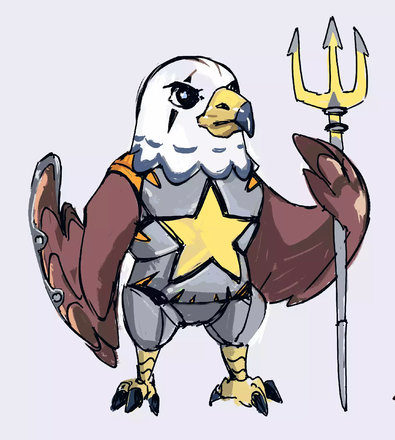
\includegraphics[width=0.2\textwidth]{Assets/ss_early}
%TODO replace image
\end{center}

\bblu{Camoragi}, the biggest idol of the Cosmooverse, also makes an appearance. She mainly sings for the government, but never hesitates to sing for its enemies. Incredibly versatile, you will also hear her in `How June and Ru D. Met'.\\

\begin{center}

\includegraphics[width=0.3\textwidth]{Assets/camo-small}
\end{center}

%\AddToShipoutPictureBG*{\includegraphics[width=\paperwidth,height=\paperheight]{cover_fx_1}}
\clearpage 

\bo{`How June and Ru D. Met'} celebrates Ru D.'s first steps into rebellion. 

Initially on a government mission, Ru D. is tricked by evil Doctor Wing, a Chicken Fast Food Mogul and government ally who attempts to turn innocent aliens into Crispy Chicken Wings, framing Ru D. for the crime. While escaping Ru D. meets June, together they save the aliens and neutralize Wing thanks to June's updated invention, the `Crispy Again Gun'.

Shoot once and your target is 10 minutes younger, shoot twice and it becomes as young as a newborn.\\

\bblu{June} is an inventor imprisoned and exploited by Doctor Wing to engineer everlasting Crispy Chicken. She is not only a genius scientist, but also a self-proclaimed accomplished musician.

\begin{center}

\includegraphics[width=0.2\textwidth]{Assets/june-head}
%
\includegraphics[width=0.2\textwidth]{Assets/june-head.webp}
\end{center}



\clearpage